% This file was created by tikzplotlib v0.9.5.
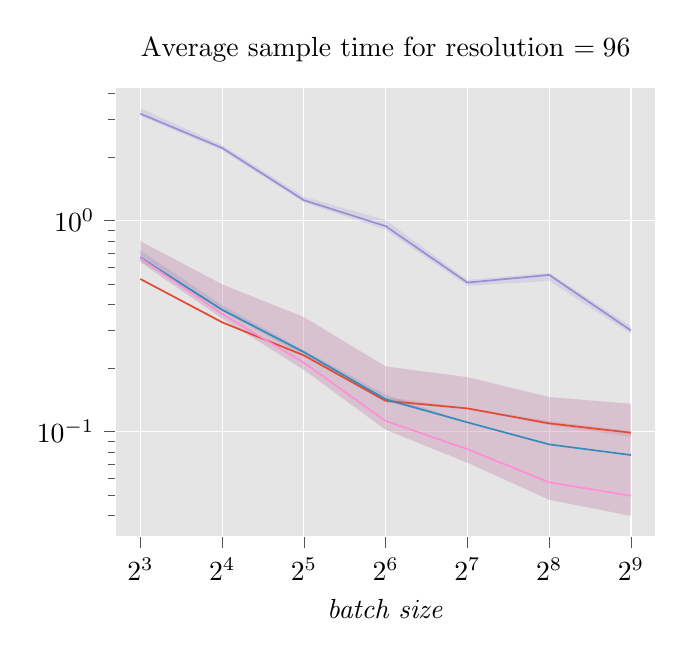
\begin{tikzpicture}

\definecolor{color0}{rgb}{0.886274509803922,0.290196078431373,0.2}
\definecolor{color1}{rgb}{0.203921568627451,0.541176470588235,0.741176470588235}
\definecolor{color2}{rgb}{0.596078431372549,0.556862745098039,0.835294117647059}
\definecolor{color3}{rgb}{0.984313725490196,0.756862745098039,0.368627450980392}
\definecolor{torchscript}{rgb}{0.996078431372549,0.556862745098039,0.835294117647059}

\begin{axis}[
axis background/.style={fill=white!89.8039215686275!black},
axis line style={white},
%legend cell align={left},
%legend style={fill opacity=0.8, draw opacity=1, text opacity=1, draw=white!80!black, fill=white!89.8039215686275!black},
log basis y={10},
tick align=outside,
tick pos=left,
title={Average sample time for resolution $=96$},
x grid style={white},
xlabel={\textit{batch size}},
xmajorgrids,
xmin=2.7, xmax=9.3,
xtick style={color=white!33.3333333333333!black},
y grid style={white},
%ylabel={time (ms)},
ymajorgrids,
ymin=0.0318818812180445, ymax=4.24381955156468,
ymode=log,
ytick style={color=white!33.3333333333333!black},
xticklabels={$2^3$, $2^4$, $2^5$, $2^6$, $2^7$, $2^8$, $2^9$},
xtick={3,...,9},
]
\path [fill=color0, fill opacity=0.2, very thin]
(axis cs:3,0.532711)
--(axis cs:3,0.525274)
--(axis cs:4,0.325467)
--(axis cs:5,0.227339)
--(axis cs:6,0.137164)
--(axis cs:7,0.127286)
--(axis cs:8,0.107328)
--(axis cs:9,0.0943382)
--(axis cs:9,0.100206)
--(axis cs:9,0.100206)
--(axis cs:8,0.1119)
--(axis cs:7,0.129387)
--(axis cs:6,0.145102)
--(axis cs:5,0.230137)
--(axis cs:4,0.333086)
--(axis cs:3,0.532711)
--cycle;

\path [fill=color1, fill opacity=0.2, very thin]
(axis cs:3,0.7206)
--(axis cs:3,0.643425)
--(axis cs:4,0.371694)
--(axis cs:5,0.227935)
--(axis cs:6,0.138768)
--(axis cs:7,0.110285)
--(axis cs:8,0.0866569)
--(axis cs:9,0.0769451)
--(axis cs:9,0.077837)
--(axis cs:9,0.077837)
--(axis cs:8,0.0870269)
--(axis cs:7,0.110558)
--(axis cs:6,0.149246)
--(axis cs:5,0.242581)
--(axis cs:4,0.39549)
--(axis cs:3,0.7206)
--cycle;

\path [fill=color2, fill opacity=0.2, very thin]
(axis cs:3,3.397831)
--(axis cs:3,3.123268)
--(axis cs:4,2.145072)
--(axis cs:5,1.215587)
--(axis cs:6,0.90215)
--(axis cs:7,0.489502)
--(axis cs:8,0.516421)
--(axis cs:9,0.290157)
--(axis cs:9,0.314908)
--(axis cs:9,0.314908)
--(axis cs:8,0.564356)
--(axis cs:7,0.522439)
--(axis cs:6,1.003318)
--(axis cs:5,1.29437)
--(axis cs:4,2.273831)
--(axis cs:3,3.397831)
--cycle;

\path [fill=white!46.6666666666667!black, fill opacity=0.2, very thin]
(axis cs:3,0.797093)
--(axis cs:3,0.633669)
--(axis cs:4,0.342584)
--(axis cs:5,0.195655)
--(axis cs:6,0.101828)
--(axis cs:7,0.071068)
--(axis cs:8,0.0474417)
--(axis cs:9,0.0398198)
--(axis cs:9,0.13526)
--(axis cs:9,0.13526)
--(axis cs:8,0.145412)
--(axis cs:7,0.180774)
--(axis cs:6,0.20295)
--(axis cs:5,0.348112)
--(axis cs:4,0.497252)
--(axis cs:3,0.797093)
--cycle;

\path [fill=torchscript, fill opacity=0.2, very thin]
(axis cs:3,0.797093)
--(axis cs:3,0.633669)
--(axis cs:4,0.342584)
--(axis cs:5,0.195655)
--(axis cs:6,0.101828)
--(axis cs:7,0.071068)
--(axis cs:8,0.0474417)
--(axis cs:9,0.0398198)
--(axis cs:9,0.13526)
--(axis cs:9,0.13526)
--(axis cs:8,0.145412)
--(axis cs:7,0.180774)
--(axis cs:6,0.20295)
--(axis cs:5,0.348112)
--(axis cs:4,0.497252)
--(axis cs:3,0.797093)
--cycle;

\addplot [semithick, color0]
table {%
3 0.527113080024719
4 0.328776597976685
5 0.229123681783676
6 0.139674320816994
7 0.128557801246643
8 0.10912749171257
9 0.098616324365139
};
%\addlegendentry{cudnn}
\addplot [semithick, color1]
table {%
3 0.66579794883728
4 0.376946628093719
5 0.237425118684769
6 0.141885712742805
7 0.110373191535473
8 0.0867782235145569
9 0.077290840446949
};
%\addlegendentry{libtorch}
\addplot [semithick, color2]
table {%
3 3.20224666595459
4 2.2035346031189
5 1.24600088596344
6 0.938888311386108
7 0.50709193944931
8 0.551432967185974
9 0.300852745771408
};
%\addlegendentry{pytorch}
\addplot [semithick, torchscript]
table {%
3 0.662334620952606
4 0.360176265239716
5 0.211528897285461
6 0.112016521394253
7 0.0824229493737221
8 0.0573519766330719
9 0.0495683811604977
};
%\addlegendentry{torchscript}
\end{axis}

\end{tikzpicture}
